\subsection{Evaluation}
\label{sec:evaluation}

\begin{figure}
	\vspace*{-\figskipabove px}
	\centering
	\hspace*{-4px}
	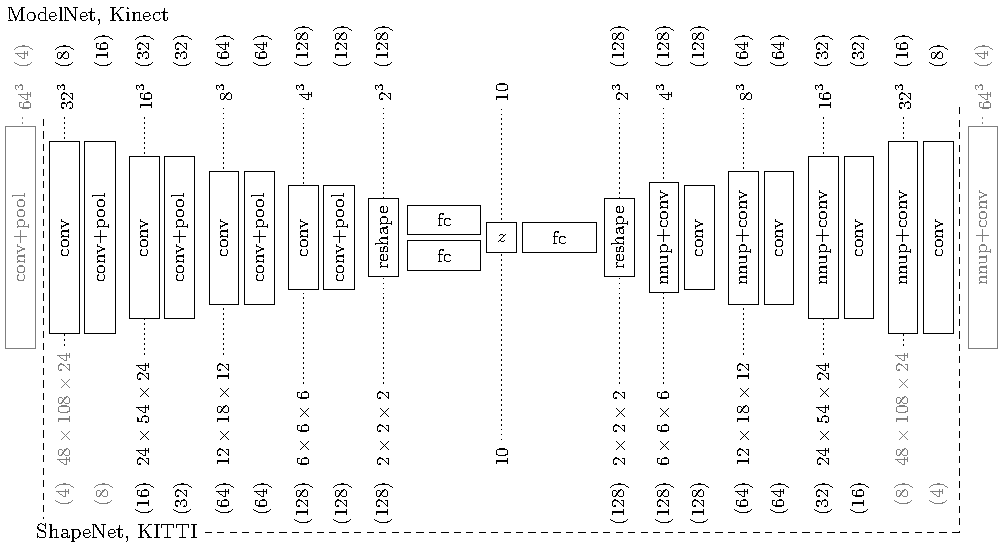
\includegraphics[width=1.025\linewidth]{fig_architectures}
	\vspace*{-12px}
	\caption{{\bf Network Architectures.} We use different resolutions for ShapeNet and KITTI as well as ModelNet and \Kinect (bottom and top, respectively). In both cases, architectures for higher resolutions employ one additional stage in the en- and decoder (in {\color{gray}gray}). Each convolutional layer is followed by $\text{ReLU}$ activations and batch normalization \citep{Ioffe2015ICML}; the window sizes for max pooling and nearest-neighbor upsampling can be derived from the context; the number of channels are given in parentheses.}
	\label{fig:architectures}
	\vspace*{-\figskipbelow px}
\end{figure}

For occupancy grids, we use Hamming distance (\Abs) and intersection-over-union (\IoU) between the (thresholded) predictions and the ground truth; note that lower \Abs is better, while lower \IoU is worse. For SDFs, we consider a mesh-to-mesh distance on ShapeNet and a mesh-to-point distance on KITTI. We follow \citep{Jensen2014CVPR} and consider accuracy (\Acc) and completeness (\Compl). To measure \Acc, we uniformly sample roughly $10\text{k}$  points on the reconstructed mesh and average their distance to the target mesh. Analogously, \Compl is the distance from the target mesh (or the ground truth points on KITTI) to the reconstructed mesh. Note that for both \Acc and \Compl, lower is better. On ShapeNet and ModelNet, we report both \Acc and \Compl in voxels, \ie, in multiples of the voxel edge length (\ie, in [vx], as we do not know the absolute scale of the models); on KITTI, we report \Compl in meters (\ie, in [m]).